\documentclass[11pt]{article}

\usepackage{url}
\usepackage{hyperref}
\usepackage{graphicx}
\usepackage{upquote}
%\usepackage{float}
\setlength{\parskip}{0.5cm plus4mm minus3mm}

\usepackage[margin=1in]{geometry}
%\textwidth=6.4in \textheight=8.5in \hoffset=-0.7in \voffset=-0.7in

\setlength{\parindent}{0cm}
\setcounter{tocdepth}{1}

\hyphenation{Text-Wrangler}

\title{GPR data processing and visualization with GPR-O}

\author{Alain Plattner (\url{plattner@alumni.ethz.ch})\\Austin Robbins (\url{austin.r.robbins@gmail.com})}

\date{\today} 
  
\begin{document}
\maketitle 
\tableofcontents
\section{General remarks}

You can download Octave for free from
\url{https://www.gnu.org/software/octave/}

If you already possess Octave, we recommend updating to the current version,
to avoid potential issues with package installation.

In the following, whenever we say ``run xxxx'' we mean in Octave or
Matlab, type xxxx and press enter.

Whenever you use an Octave (or Matlab) program for the first time, for
example by the name xyz, run
 
\qquad \verb#help xyz#
 
This will display the required input(s) and show the output(s) of that
program or function. In general, well-documented programs will also provide
a description of what the function does. 

For all GPR-O programs to run, your current directory (shown at the
top of your Octave or Matlab program window) must be the GPR-O
folder. If you are an advanced user, you can add all the subfolders to
your Octave or Matlab path.

In the command window you can recall previously entered commands by
pressing the up and down keys and you can let the computer suggest
completions of commands with the tab key.

\section{GPR-O installation}

If you have yet to install GPR-O (you downloaded the documentation only),
follow the installation instructions here

\url{https://github.com/NSGeophysics/GPR-O}

Once you have downloaded the GPR-O program files and folders, run, in
Octave or Matlab (in the GPR-O folder)

\qquad \verb#setup#

This will download some external program files that are necessary to
run GPR-O.

Keep your software and this documentation updated by regularly running, in a
command prompt/terminal in the folder GPR-O

\qquad \verb#git pull origin master#


\section{Data structure and data preparation}

To use GPR-O, switch to the GPR-O folder on your computer. This folder
contains a few subfolders and a few m-files. Each m-file is a computer
program that was written for Octave (or Matlab; they are, for our
programs here, interchangeable).

If you are using Matlab, to access to all the subprograms you need to run

\qquad \verb#initialize#

If you are using Octave, run

\qquad \verb#initialize_octave#

The first time you run this initialization, it will check if
all required Octave packages are already installed and if not, will
automatically install them. This may take a few minutes. Next time you
run it, it will not need to install the packages anymore.

We will use a variety of programs that are stored in the
subfolders. Whenever you want to know what a program does and what
variables you need to give it, run ``help programname''. For example,
we have a program that is named ``\verb#readdata#''. To find out how to use
it, run

\qquad \verb#help readdata#

Octave will show you a text saying from where the function is stored, what
input it requires, and what output it gives.

For the required input, the help page says:

\verb#surveyparams# A struct with the following fields:
%\vspace{-0.5cm}
\begin{itemize}
\item \verb#nlines# Lowest line number
\item \verb#nmorelines# Would be 3 if you had 4 parallel line with the numbers 0 1 2 3
\item \verb"lineincr" The distance between the lines (in meters)
\item \verb#pnameraw# String containing the directory of the raw files dt1
\item \verb#pnametrf# String containing the directory for the processed files
\end{itemize}
 
This variable named \verb#surveyparams# will play a key role in
GPR-O. For each survey you will need to set it up. This is easily
done by writing your own m-file as described in the following.

Double-click on ``\verb#Example1.m#'' in the file browser directory within Matlab/Octave. 
The command window will disappear and a new window named ``Editor'' will appear.

On the first line of the script, you will see ``surveyparams.minline=0;'' 
and then a percent sign and then some comment. This tells GPR-O that the 
first data file to call will have a value of zero in the filename, such as ``XLine00''.
If the first line of your data set starts with, for example, ``XLine02'',
then you would enter a ``2'' instead.

The second line says ``surveyparams.nmorelines=24;'' which means that
GPR-O will search for 24 more data files after the initial one is found.
In order to view a single line from your data, you would simply input
the line number in ``surveyparams.minline=?;'' and ``surveyparams.nmorelines=0;''.

The next line says ``surveyparams.lineincr=0.2;''. This means that the
distance between each profile line is 0.2 m.

The following line says
``surveyparams.pnameraw='data/raw/example1/';''. This means that the
data that we recorded with the GPR is stored in the folder
``data/raw/example1/''. Open that folder on your desktop and you will
see that it contains several files that are named ``XLINE00.DT1'' etc,
and ``XLINE00.HD'' etc. These are data files from an actual GPR survey 
and we will be working with these as an example. For your own data files 
you will create a folder besides the ``exercise1'' etc folders in the data 
directory and store your GPR files in there.

The last line in ``example1.m'' says
``surveyparams.pnametrf='data/processed/example1/';''. This means that
the processed data will be stored in the folder
``data/processed/example1/''. If you open, on your desktop, the folder
``'data/processed', then you will see that it is empty. We need to
create this folder to continue. \textbf{If you don't create this folder
  the program will create an error when you try to pre-process the
  data. So make a folder ``example1'' in the directory ``processed''.}

For your own data you must create your own m-file (just overwrite 
``example1.m'' with a new file name and your particular survey parameters).
Also, you must ensure that you created the proper folder structure 
that corresponds to your m-file.

\section{Data preprocessing and data loading}
\emph{To return to the Command Window when the Editor is visible,
  click on the tab at the bottom of the Octave program window.}

Once you have set up the folder structure and the m-file for your
data, you can, back in the Command Window, set the ``surveyparam''
variable by running

\qquad \verb#example1#

or whatever the name of your m-file is. Notice that running your program
loads the ``surveyparam'' variable into the workspace. You can display the
components of the surveyparams variable by running

\qquad \verb#surveyparams#

This should show you all the information you previously put into your
m-file.  Now run

\qquad \verb#preprawdata(surveyparams)#

to preprocess your data. If it doesn't work it is likely that you made
one of the following mistakes:
\begin{itemize}
\item You did not enter the correct folder for your raw data in your
  m-file
\item you did not enter the correct folder for your processed data in
  your m-file, or you did not create that folder
\item when collecting the GPR data, you did not select ``record grid
  data'' and then ``X-lines''. You can see this by looking at your raw
  data folder. If the files say ``YLINE00.DT1'' etc, or just
  ``LINE00.DT1'' etc, then that's what happened. No worries, in that
  case you can just run \qquad \verb#preprawdata(surveyparams,1)# if
  the names are ``YLINE00.DT1'', or \verb#preprawdata(surveyparams,2)#
  if the names are ``LINE00.DT1''.
\end{itemize}

After successfully preprocessing the data, you can load it by running

\qquad \verb#data=readdata(surveyparams);#

The semicolon at the end is necessary to avoid that your screen gets
filled up with numbers. If that happens you can press ``ctrl-c'' to
abort and run it again with the semicolon.
 
The ``data=readdata(surveyparams)'' command takes the variable structure
``surveyparams'' as input for the function ``readdata'', and stores the 
data as the variable ``data'' in the workspace.

\section{Profile data plotting and processing}\label{secProfiles}

\subsection{Plotting the raw data}

Let's have a look at the data you just loaded. Remember that we have
25 parallel lines that are numbered from 0 to 24. We can plot the
first line (number 0) by running

\qquad \verb#plotGPRline(data,0);#


It should look something like
\begin{center}
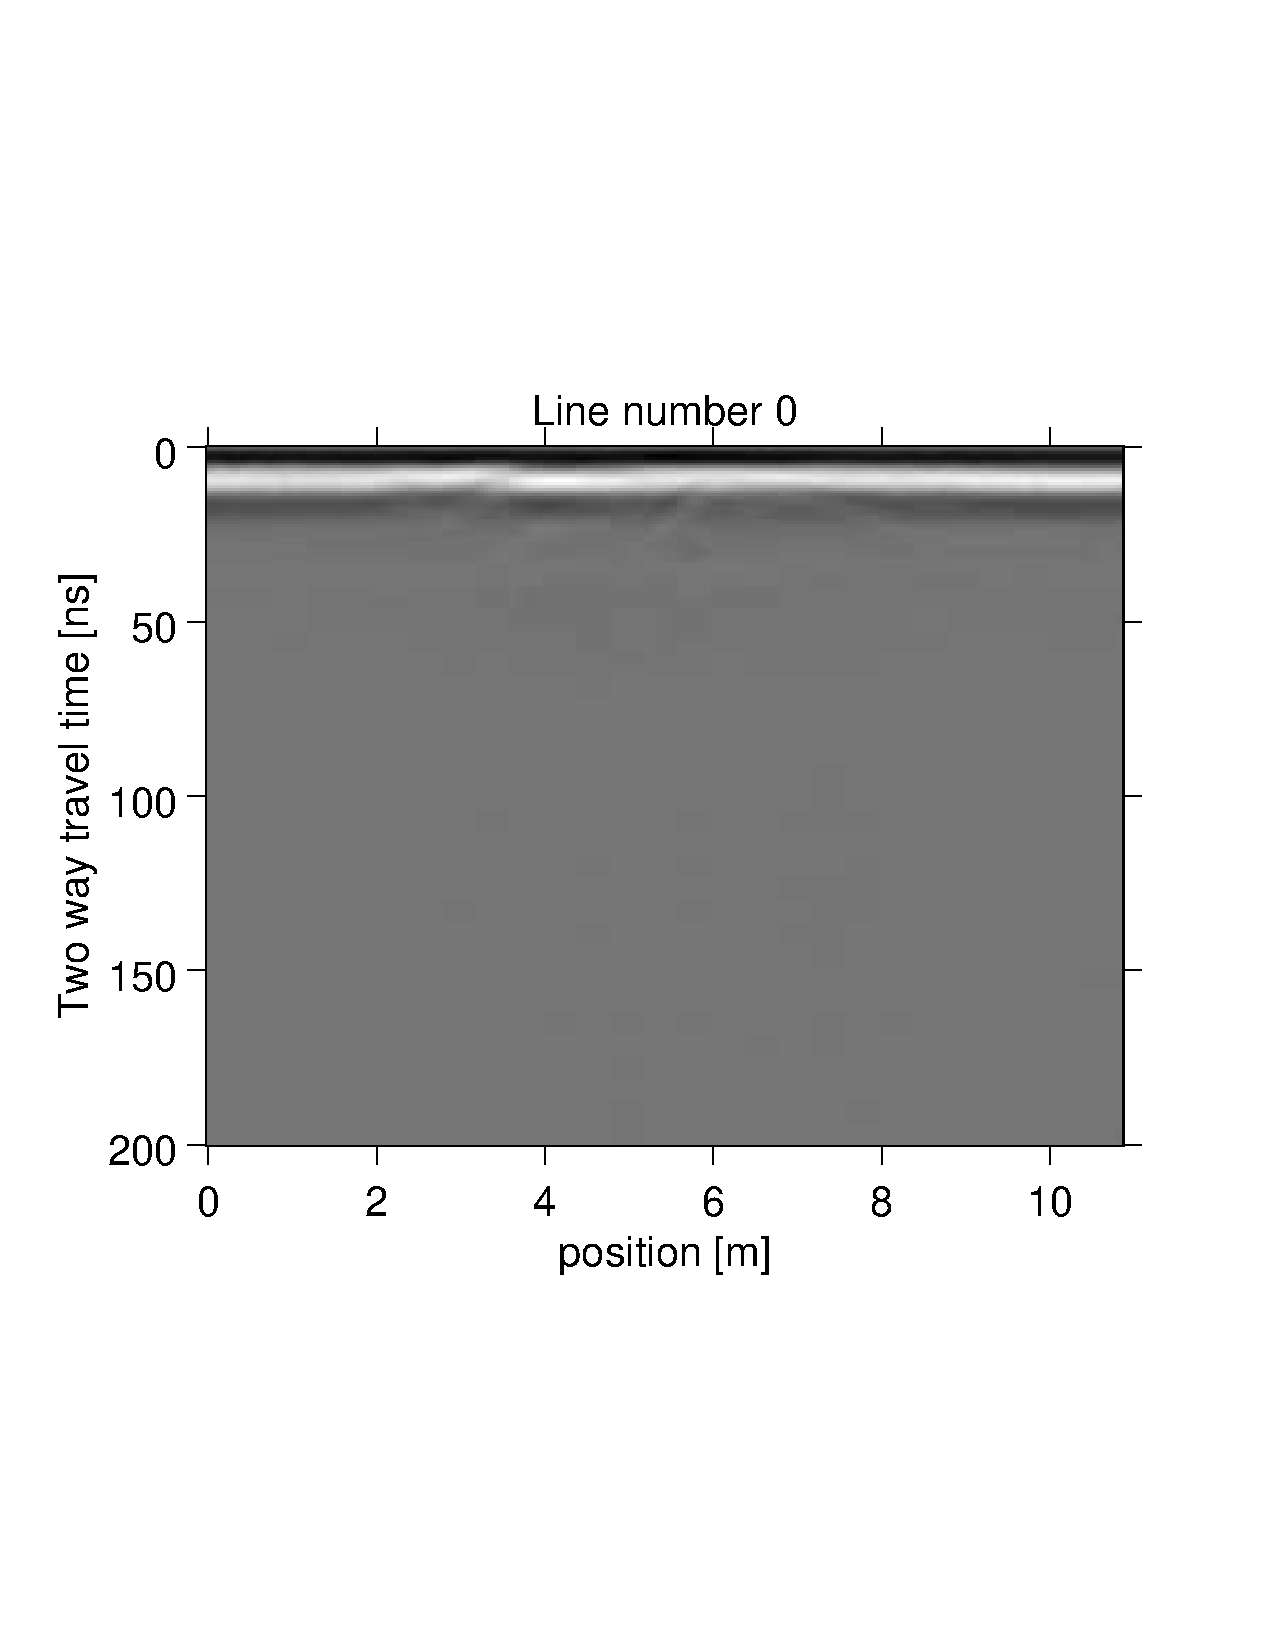
\includegraphics[width=0.7\textwidth, trim = 0.9cm 6cm 2cm
  6.5cm,clip]{figures/GPRline0}
\end{center}

Notice the function ``plotGPRline'' requires two inputs. The first
is the variable that contains the processed data, in our case ``data''.
The second refers to which line we wish to plot. So, if you want to show the second line, run 
\qquad \verb#plotGPRline(data,1);#,
\\and for the third line
\qquad \verb#plotGPRline(data,2);#, etc.
 
You can always export a figure as pdf by clicking, in the figure
window, on ``File'' and then ``Save As''.

What this figure shows is: along the first profile, at every location,
the GPR sent out a wave and recorded what came back (as a function of
time). This wave is shown as a row of pixels in grayscale going from
the top to the bottom. The way we obtain a full 2D image instead of
just a single wave signal is that we plot all of these lines next to
each other.

In this profile we did not see much else but the black and white
horizontal stripes in roughly the first 12 nanoseconds. This is
because the wave that left the transmitter antenna flew directly into
the receiver antenna without going through the ground. This wave is
called \emph{air-wave}. In this setup, the antennae were 0.5 m apart
and the frequency was 100 MHz. A radar wave moves with the speed of
light. In air this is roughly 0.3 m/ns. A wave of this frequency has
length $0.3*10^9$ m/s divided by $100*10^6$ 1/s, which is 3 m. For the
entire 3 m wave to completely pass by the receiver antenna located 0.5
m away, the wave needs to travel 3.5 m. At the speed of light, it takes this
wave 3.5 m divided by 0.3 m/ns, which is 11.67 ns, exactly the time
where we see the black and white stripe end.

\subsection{Removing the air-wave}

So we just saw that our image is dominated by the radar wave traveling
through air and we don't see much from the waves traveling through
ground (which are slower but also more weakened when they travel
through the ground). We therefore want to remove the air-wave to see
what is in the ground. Because the distance between the antennae is
always the same in this profile (they were fixed at 0.5 m apart), the
air-wave always looks the same at each recorded position (in each
trace). On the other hand, the subsurface will vary along our profile
unless there is a perfectly horizontal object in the subsurface all
the way from the first to the last recorded position (which is rarely
the case but can happen, so keep this in mind when doing this
processing step). If the subsurface does not look the same all the way
from the first to the last recorded position, but the air-wave does,
then the average of all recorded traces should look like like the
air-wave. Therefore if we average the traces for all recorded
positions and subtract the result from each trace, then we should be
able to remove the air-wave but keep all the signals from the
subsurface. We can do this with the function
\verb#removeHorizontal#. Run

\qquad\verb#dataH=removeHorizontal(data,10000);#

This creates a new variable ``dataH'' which now has the air-wave
removed. We needed to give the program the number of measurement
locations it should use to average. By giving it a very high number,
say ``10000'' we just average all locations per profile. The less
locations you average, the more aggressively you remove horizontal
features. The most extreme is if you say 1, because then you remove
everything and end up with no signal at all.

Let's see how the processed data looks like. Run

\qquad \verb#plotGPRline(dataH,0);#

\clearpage
It should look something like

\begin{center}
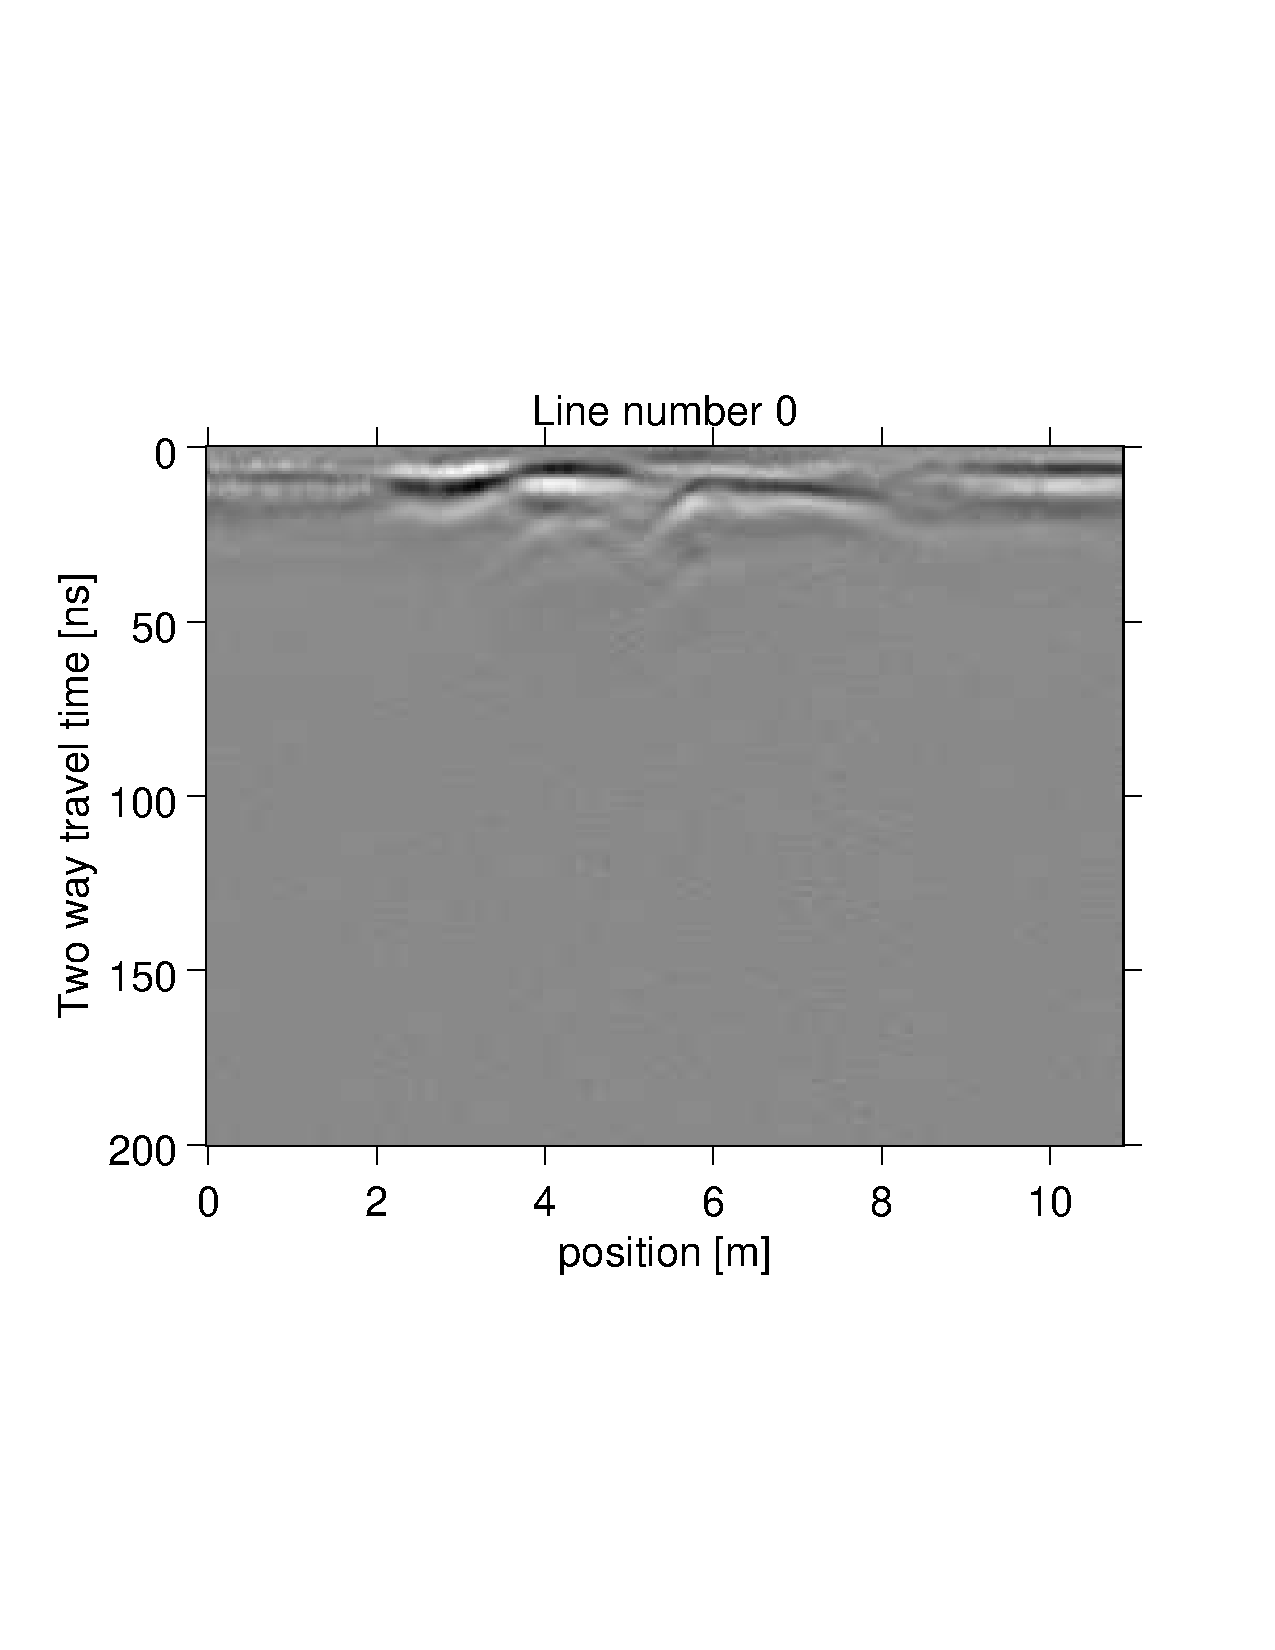
\includegraphics[width=0.7\textwidth, trim = 0.9cm 6cm 2cm
  6.5cm,clip]{figures/GPRlineH0}
\end{center}
 
Much better. We can actually see something. But everything we see is
at early, two-way travel times and therefore close to the surface. Why
could that be?

\subsection{Gaining the data}

Radar waves traveling through ground (as opposed
through air or space) are weakened (attenuated) quite
quickly. That means that the deeper down the wave travels, the weaker it
becomes, and therefore we can't really see much when it gets bounced off an
interface in the subsurface and comes back to the surface.
 
But there is a way to make these deeper signals more visible. We can
artificially strengthen later travel times by multiplying them with an
increasing factor. This is called ``gaining the data'', or ``applying
gain''. GPR-O presently has two different ways of gaining the data and
:\verb#gainDataTPOW# and \verb#gainDataAGC#. The method you choose depends
upon your data and your target of interest.


\subsubsection{t-power gain (TPOW)}

The simplest way of increasing the strength of the displayed data with
depth is to just multiply greater depths with large numbers and
shallow depths with small numbers. At this point, we are still looking
at position vs two-way travel time (at a later point we will, for
constant subsurface velocities, display the data as position vs
depth). Therefore, we do not increase the strength of the signal along
the depth axis, but along the two-way-travel-time-axis. A simple but
flexible way of increasing strength with two-way-travel-time $t$ is to
just multiply each trace with a power of $t$, so multiply with $t^a$
and we can choose $a$. So if we say for example $a=1$, then we
increase strength linearly with $t$. If we say $a=2$, then we increase
strength with the square of $t$, etc. We can also say $a=1.3$ for
example, or $a=0.3$, or even negative values for $a$. If we use $a=0$
then we do nothing with the data and the result looks the same as
without gaining. If we use a negative $a$, then we increase the strength
close to the surface and decrease the strength further away (which is
usually not what we want).

Let's try this with our data set. For example, let's choose
$a=0.85$. This means we have to run

\qquad \verb#dataHGt=gainDataTPOW(dataH,0.85);#

To plot the first line we run

\qquad \verb#plotGPRline(dataHGt,0);#

The result should look like

\begin{center}
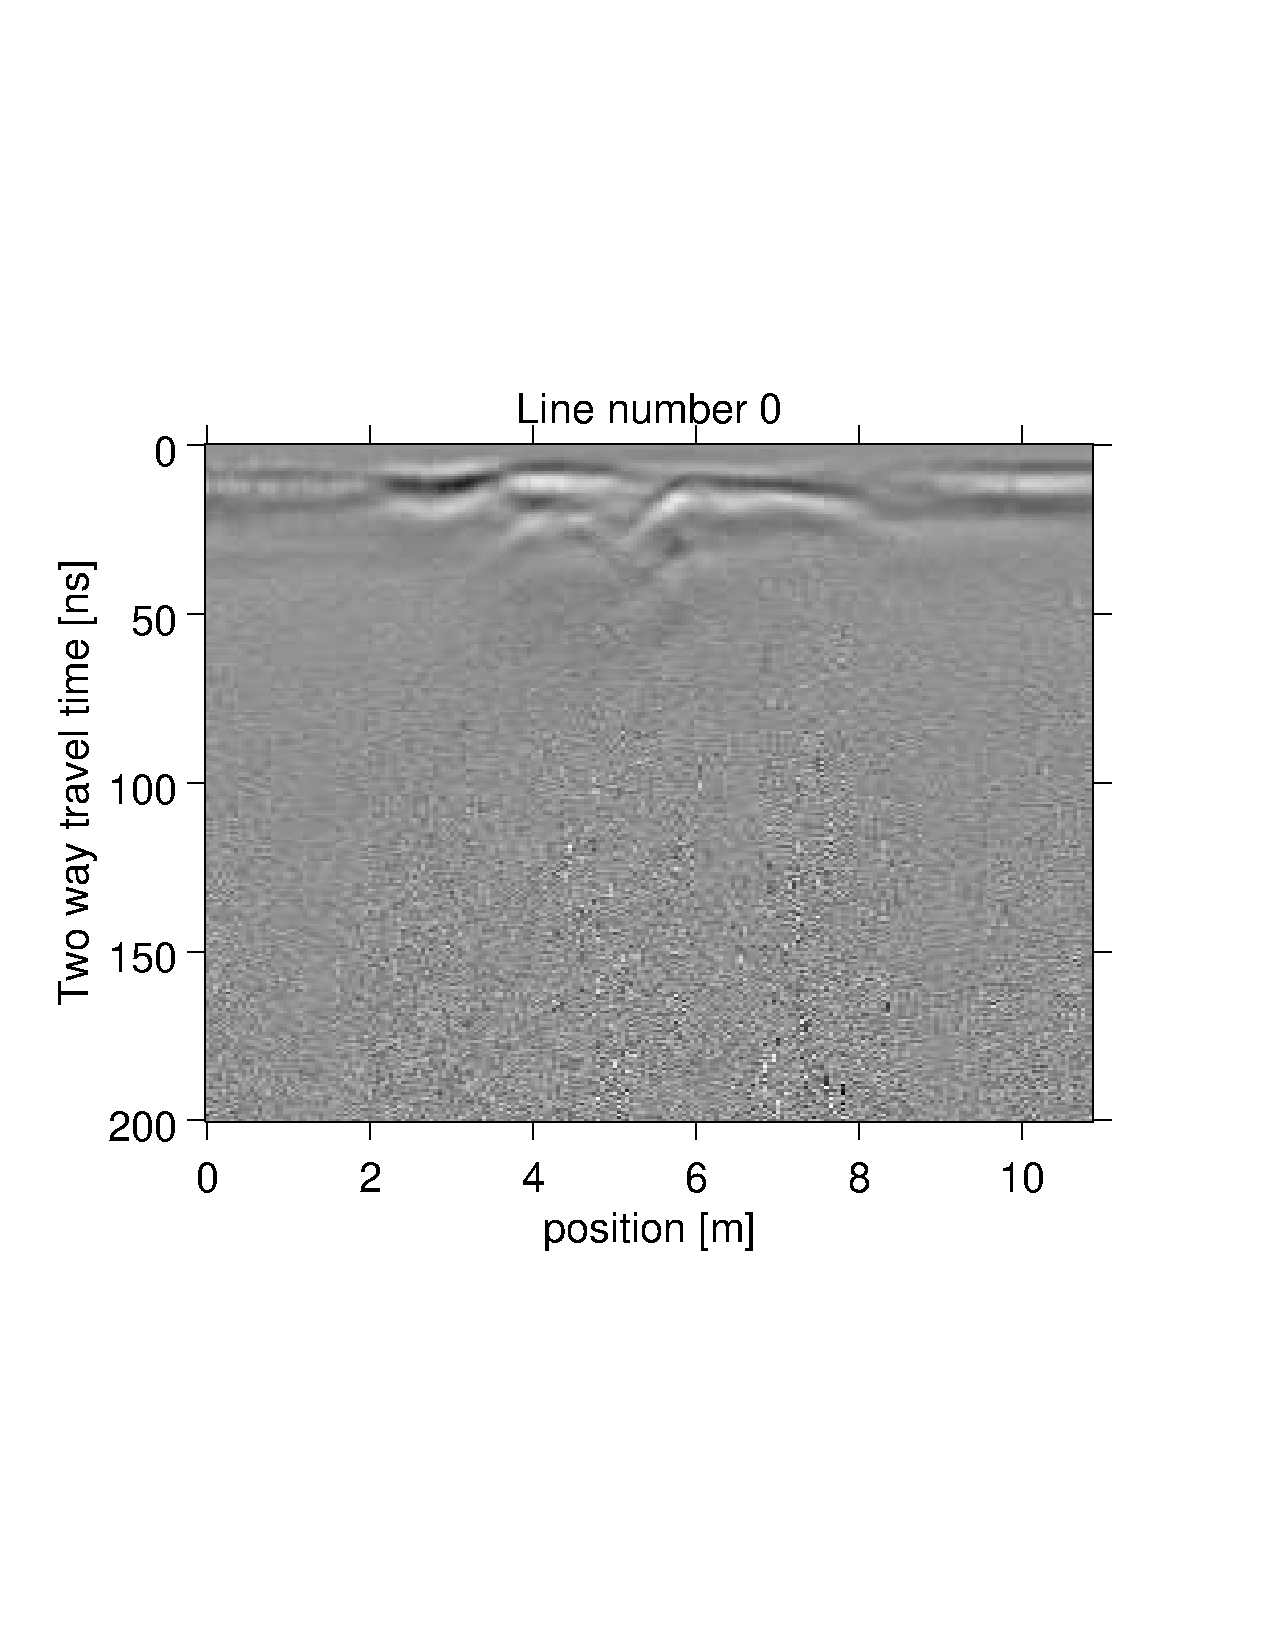
\includegraphics[width=0.7\textwidth, trim = 0.9cm 6cm 2cm
  6.5cm,clip]{figures/GPRlineHGt0}
\end{center}

This looks very similar to the data with just the air-wave
removed. The difference is that the objects deeper down (just above 50
ns) now look a bit stronger and the shallower objects look a bit
weaker. For this (admittedly not very exciting) data set, the t-power
gain is not very helpful but for other data sets, where you have
interesting objects deeper down, the t-power gain may be superior to
other gains. Generally, when playing with gain it is worthwhile to try
out different settings. A good philosophy is that you want to enhance
the target objects you are looking for if they are also in the raw
data, but you do not want to use processing to create objects that are
not really in the raw data. While appropriate gaining will provide the
best results from a data set, such processing should never replace
thoughtful survey design (i.e. antennae frequency selection). 

\subsubsection{Automated gain control (AGC)}

Instead of using a simple power law to increase the strength of the
signal at greater depth (later two-way travel time), we could also say
that we want the signal to have about the same strength at all
depths. One way of doing it is to define a time (depth) window and say
that the energy of the signal should be the same within each
window. For this we only need to give a window width (in number of
time-samples). Let's say that each measurement, or trace, within the profile is 
composed of 300 time-samples (for a depth resolution of 300 pixels).
By using a 5 time-sample window width, AGC forces each of the (300/5)= 60
depth intervals (or 5-sample window) to have the same power.
To do that, run
 
\qquad \verb#dataHGa=gainDataAGC(dataH,5);#

Let's see how the profile looks like after applying
AGC. Run

\qquad \verb#plotGPRline(dataHGa,0);#

It should look something like
\begin{center}
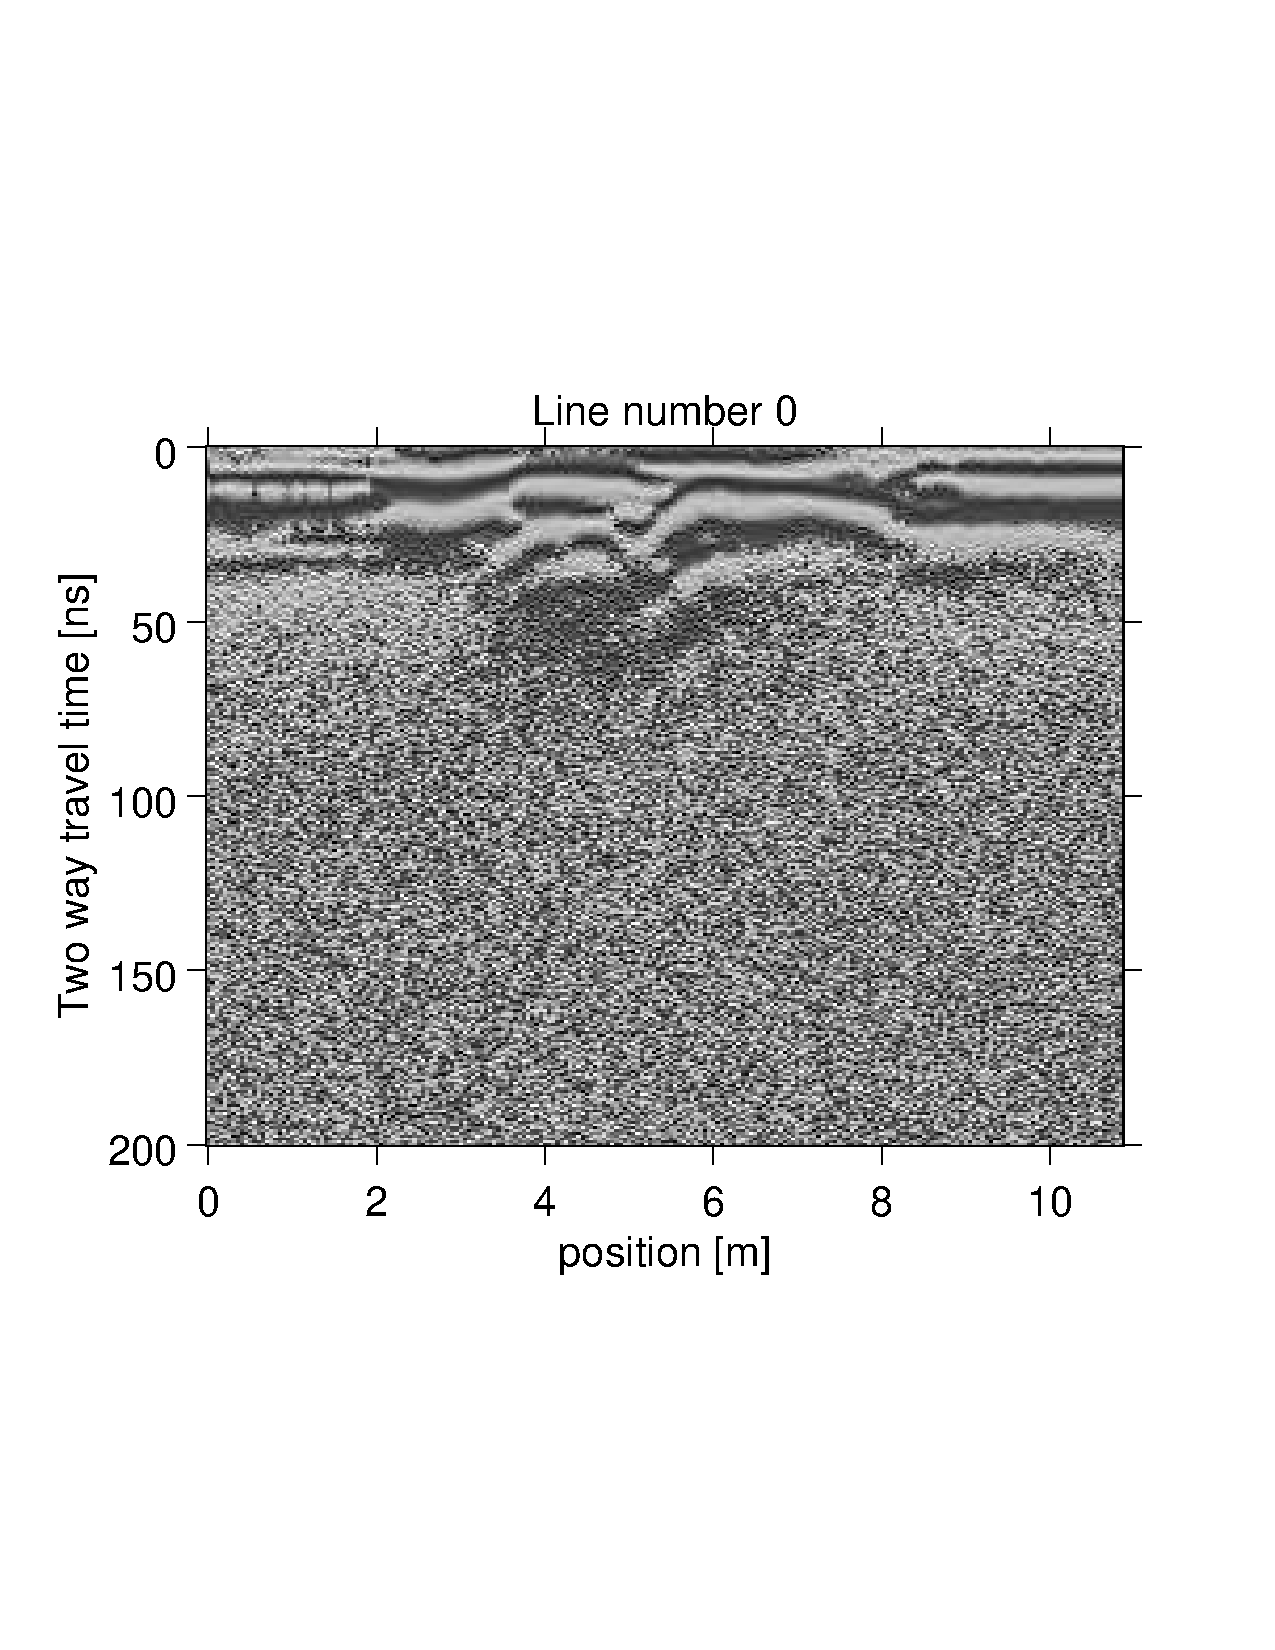
\includegraphics[width=0.7\textwidth, trim = 0.9cm 6cm 2cm
  6.5cm,clip]{figures/GPRlineHGa0}
\end{center}

The application of AGC may take a while to calculate, in particular
because you apply AGC to all 24 parallel profiles of the data set. To
only apply AGC to a single profile, for example line number 0, you can
run

\qquad \verb#dataHGa=gainDataAGC(dataH,5,0);#

This is especially helpful (and time saving) when trying different
time-sample settings. Play around with the time-sample window to see
which setting helps show the target objects best.

See

\qquad \verb#help gainDataAGC#

for more information.


\subsection{Plotting with depth}

Up until now we have always plotted our profile lines as a function of
two-way travel time. But ultimately, we want to know the depth of an
object. To do that we need to know the speed of radar waves in the
ground and this depends on the ground itself. We will learn later how
to use Common Mid-Point (CMP) and Wide Aperture Reflection and
Refraction (WARR) measurements to estimate the velocity of our ground
but for now we simply use a lookup table:
  
\url{http://gpg.geosci.xyz/content/GPR/table_velocity.html}
  
If we scroll down on that page we see that clays have a velocity of
around 0.06 m/ns. We now simply use this number in the function
\verb#plotGPRline#
  
\qquad \verb#plotGPRline(dataHGa,0,[],0.06);#
  
The time axes is now a depth axes in meters. in the previous call we
needed to add the ``['' and ``]'' characters because the velocity is
the fourth input of the function \verb#plotGPRline#. The third input
would be display contrast. If we just want to go with standard display
contrast, we can use the placeholder ``[ ]'' to say just that. We
could increase the contrast by running
  
\qquad \verb#plotGPRline(dataHGa,0,3,0.06);#

Here we are assuming that the radar velocity is constant with
depth. This is of course not true. We could, for example, encounter a
situation where we have soil on top of bedrock and the two have very
different radar velocities. Time-to-depth transformations for varying
subsurface velocities are currently not implemented in GPR-O.

\subsection{Saving processed data and comparing profiles}

Some of the processing is quite fast, but the AGC can be relatively
slow. After it is finished you might want to
save your processed data such that you do not need to start all over
next time. You can save your data with the command
 
\qquad \verb#save('exercise1dataHGa.mat','dataHGa');#
 
This created a new file named ``exercise1dataHGa.mat'' in your
directory. You can also give it any other name or store any other
processed data this way. You can always load this data set now by
double clicking on it. Try first deleting everything in your current
Octave session by running
 
\qquad \verb#clear all#
 
If you would now try to redo the plots from before you would get an
error message. Now run
 
\qquad \verb#load exercise1dataHGa.mat#
 
to load it again.  The loading takes a few seconds. Try again to plot
the data as before.


\emph{Have you noticed that whenever you plotted something new, you
  just overwrote the old plot? You can avoid this by running}

\qquad \verb#figure#

\emph{to open a new figure before you plot something new.}

Let's try this to see how the profile right next to profile 0 looks
like. Open a new figure and then run

\qquad \verb#plotGPRline(dataHGa,1);#
   
When you compare the two profiles, you will probably notice that they look very
similar. That is a good sign; it means that our data measurements are
reproducible and that we didn't just record random noise.
 

\section{Area plotting}

You have now learned to process and visualize profile data. In
example1 we have 24 such profiles. We can visualize them by plotting
each of them individually but for geological interpretations it would
be good to look at them together simultaneously. We can do that by
creating a map view where we display each of these profiles as a strip
next to each other and provide the two way travel time (corresponding
to depth) for which we want to look at them. Let's say we want to cut
through all of the profiles at 17 ns two way travel time and look at
it from bird's eye perspective.

First, make sure that you have loaded or preprocessed the data and
that you have set the variable \verb#surveyparams# (you probably
deleted it earlier when you ran \verb#clear all#. You can reload it by
running \verb#example1#).

To make the bird's eye plot of a horizontal cut at 17 ns two way
travel time run

\qquad \verb#plotdata2Dgpr(dataHGa,surveyparams,17);#

It should look like this
\begin{center}
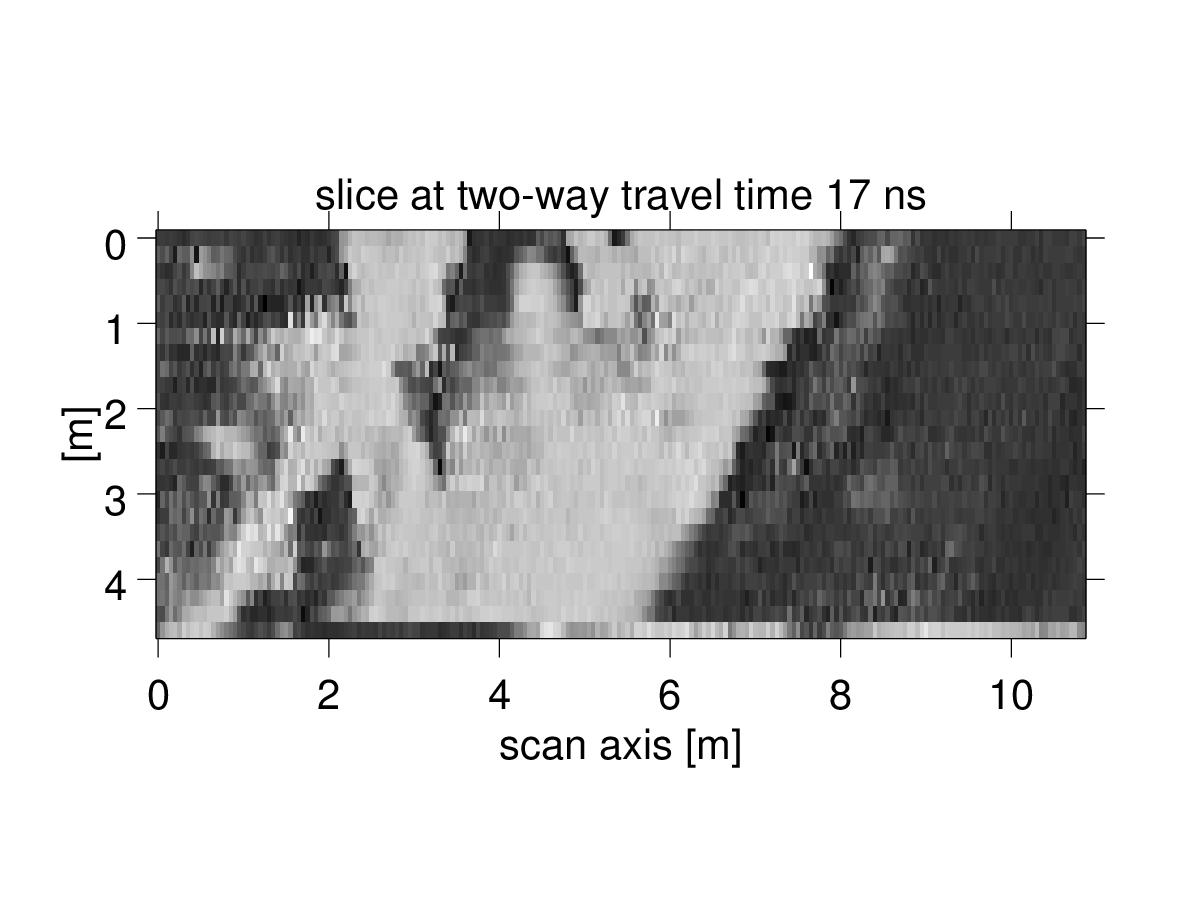
\includegraphics[width=0.7\textwidth, trim = 1cm 3cm 1cm
  3cm,clip]{figures/Area17ns.jpg}
\end{center}

The x-axis here is the along-profile axis, while the y-axis contains
the profile starting points. If your second profile is to the left of
your first profile and the third profile is to the left of the second
profile, etc, you can plot your bird's eye view with

\qquad \verb#plotdata2Dgpr(dataHGa,surveyparams,17,1);#

You will see that the entire plot is flipped.

\emph{Hint: If you save your figure as pdf, then you'll see that it will be
a bit blurry. You can avoid this by saving your figure as jpg. There
are ways to get a less blurry pdf by using the} \verb#print# \emph{function
in the Octave / Matlab Command Window.}

There is clearly a lot of structure in this depth slice. Remember that
each profile was measured independently. So structure that shows up
cross-cutting across several profile lines is some sort of
structure. But interpreting what it is is the difficult part. Let's
first get an estimation for the actual depth of this bird's eye
plot. It is at 17 ns two-way travel time, which means the signal
travelled $17/2=8.5$ ns one way. If we assume a speed of 0.06 m/ns (as
we got from the lookup table), then this will give us a depth of 8.5
ns * 0.06 m/ns = 0.51 m.

If we look at greater two-way travel times, corresponding to deeper
slices, then we see that the structure is less and less well
visible.

A slice at 30 ns should look like this
\begin{center}
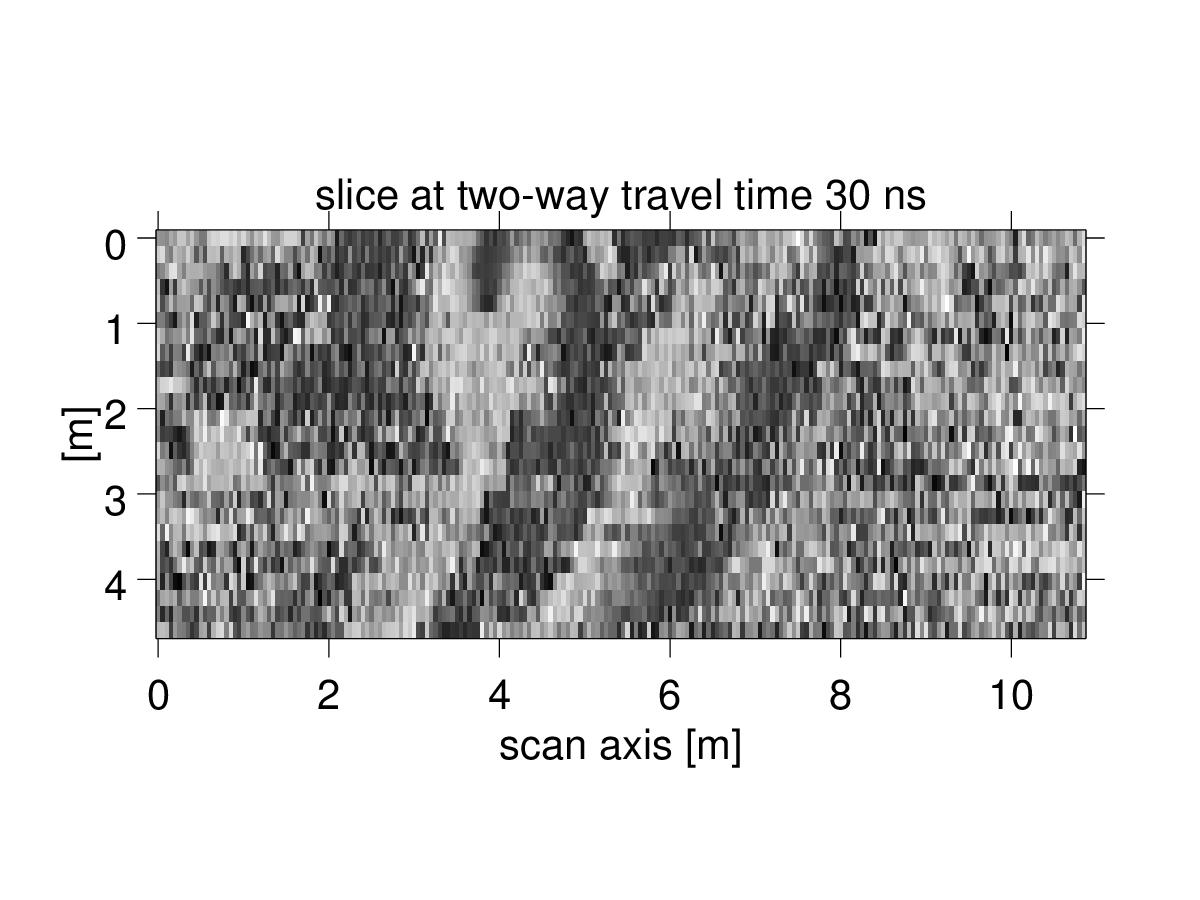
\includegraphics[width=0.7\textwidth, trim = 1cm 3cm 1cm
  3cm,clip]{figures/Area30ns.jpg}
\end{center}

We can still see some structure but there is much more noise in the
image.  \\The depth is 1/2 * 30 ns * 0.06 m/ns = 0.9 m.  Considering
that this is a 100 MHz system it is a bit disappointing that we can
only see that far. This has to do with signal attenuation (weakening)
because of the type of soil.  The soil where these data were collected
is clay-rich and is irrigated, making the subsurface rather electrically
conductive.  From general GPR theory(for example
\href{http://gpg.geosci.xyz/content/GPR/GPR_physical_properties.html}{GPG's
  GPR section}) we know that attenuation is proportional to electrical
conductivity. Therefore, in general, conductive soils are bad for GPR
depth investigations and electrically resistive soils (sand, rock,
etc) are good.


\section{CMP and WARR}

To turn travel time into depth we have so far always used a value from
a lookup table. This is based on the assumption that the velocity does
not change with depth and that we made the right guess for the soil in
the lookup table. Of course there are field-based ways of obtaining
the subsurface velocity. Two classical and very similar methods are
Common MidPoint (CMP) measurements and Wide Aperture Reflection and
Refraction (WARR). In both cases we assume that there is a subsurface
reflector that is (at least where we do our measurements) horizontal.

Here we will not go into detail about the theory of CMP and WARR
measurements but will talk about how you can use GPR-O to analyze and
visualize CMP and WARR data. We will work with the data in the folder
``example2'', which is WARR data. GPR-O has dedicated programs for
WARR and CMP. Here we will only work with the WARR programs. The CMP
programs work the same, you simply need to switch WARR with CMP such
as for example switch \verb#plotWARRhyperbola# to
\verb#plotCMPhyperbola#.

\emph{Make sure that you use the WARR programs for WARR data and the
  CMP programs for CMP data, otherwise you will get wrong velocity
  estimations}.

As before, we first need to prepare the \verb#surveyparams# variable
and the data directories. When you open ``example2.m'' you see that
the raw data directory is ``data/raw/example2/''. In that directory
you will only see a single line ``XLINE00''.

\emph{It is generally a good procedure to not mix CMP/WARR lines with
  for example GPR profiles. The reason is that when GPR-O reads the
  data it adjusts every profile such that they all have the same
  length (needed for the bird's eye slices). So if you have a 5 m CMP
  data set and a 20 m profile in the same folder, the profile will get
  truncated at 5 m. So keep them in separate folders and treat them as
  individual surveys.}

The processed directory in the m-file ``example2.m'' says
``data/processed/example2/''. If we go to the folder
``data/processed/'' we see that this folder does not yet exist. So we
need to make it.

Then, go back to the Command Window (using the tab at the bottom) and
run

\qquad \verb#example2#

and as before, prepare the raw data using

\qquad \verb#preprawdata(surveyparams)#

The data is now prepared and stored. You can now load the data with

\qquad \verb#data=readdata(surveyparams);#

Now we need the right plotting program for this WARR data set to
visualize it:

\qquad \verb#plotWARR(data)#
 

The result should be
\begin{center}
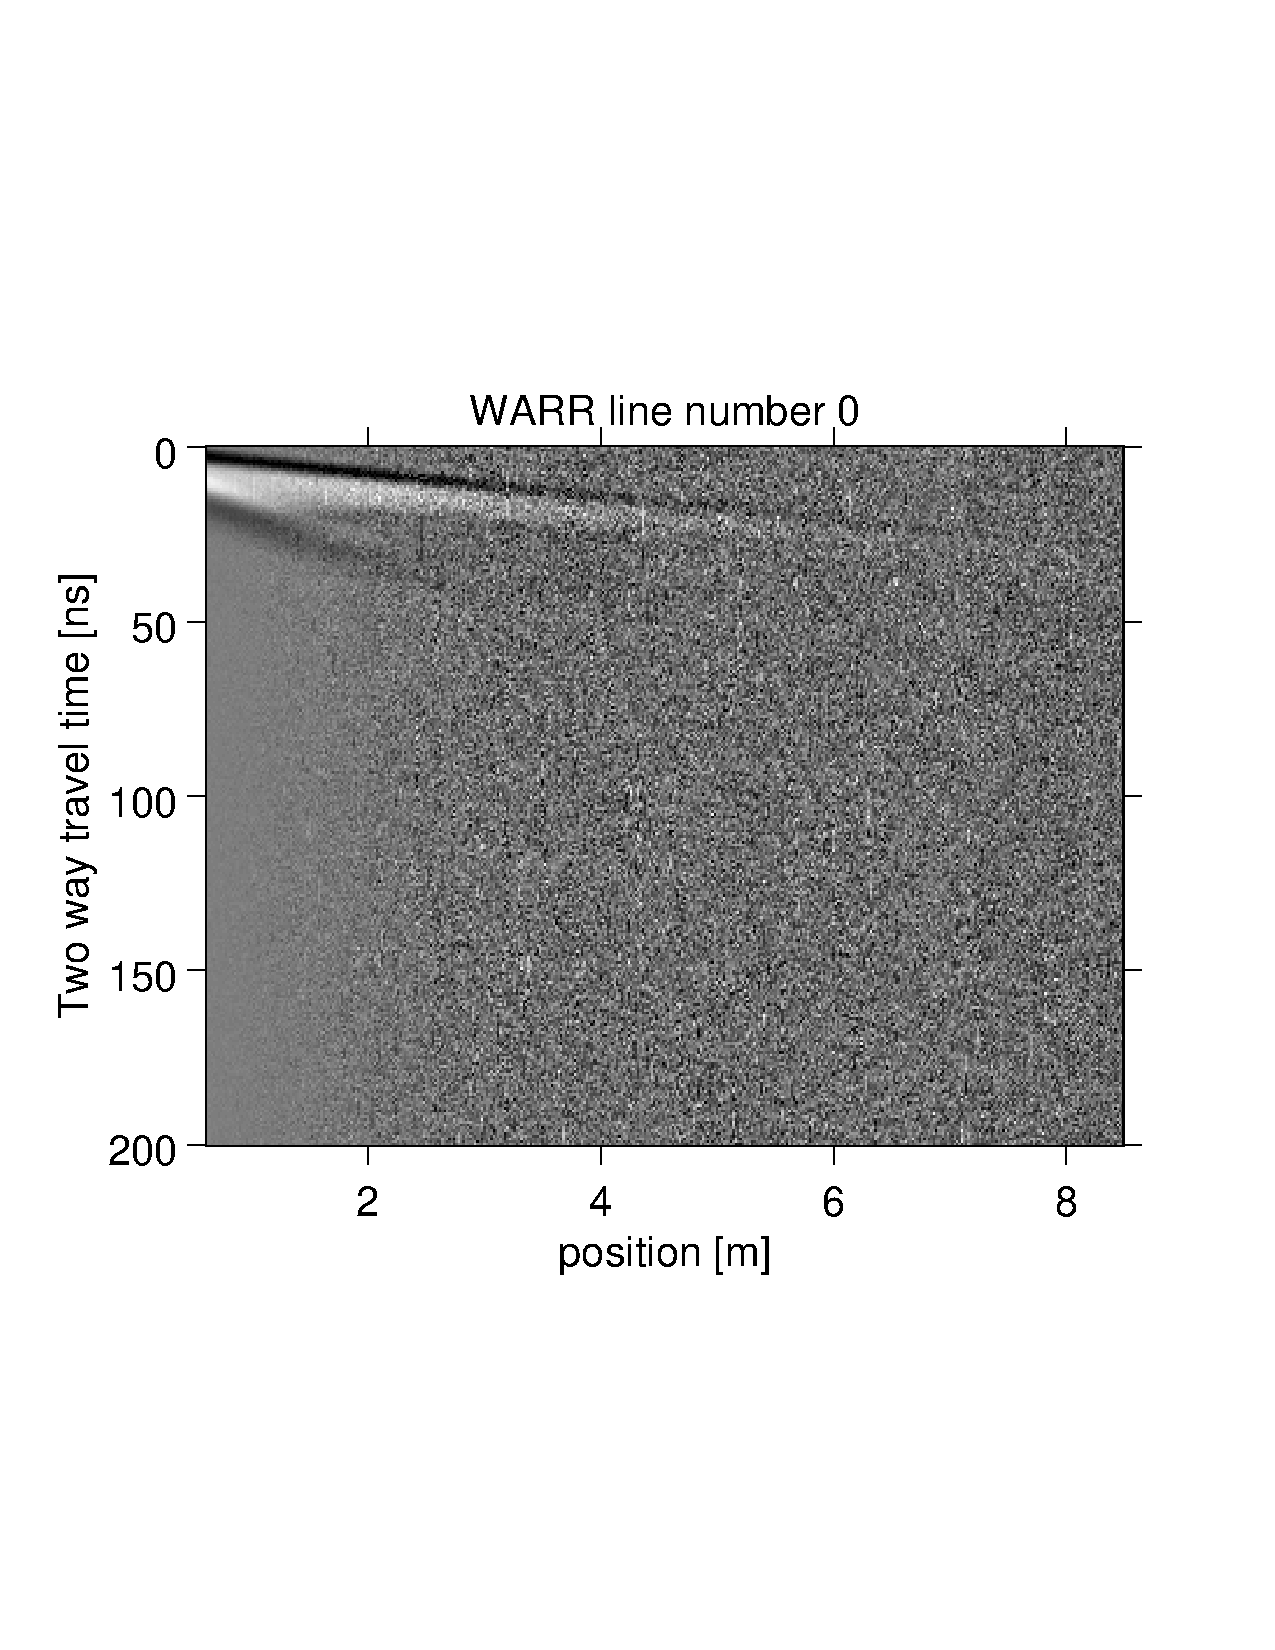
\includegraphics[width=0.7\textwidth, trim = 0.9cm 6cm 2cm
  6.5cm,clip]{figures/WARR}
\end{center}
 
What we see is, as for the GPR profiles, position versus two way
travel time. But here, position does not mean location of the GPR
system but distance between the transmitter and receiver antenna. As
you can see, the larger the antenna distance, the greater the
noise. Why would that be?
 
The answer is: the farther away the antennae are, the more the signal
gets attenuated. To compensate for that effect and to still be able to
see the signal when the antennae are 8 m apart, we amplify the
measured traces for larger antennae distances. But with that, we also
amplify the noise.
 
The following part requires you to have a basic understanding of
CMP/WARR velocity determination. If you are confused by what we do
next, please read it up in your textbook.
 
How can we obtain subsurface velocity from this WARR data set. We
could guess a velocity and whether the wave is being refracted or
reflected and then plot the corresponding line/hyperbola over the
curve to see if we are right.
 
Let's assume for now that we can see a refracted wave with velocity
0.1 m/ns that starts (for antenna distance 0 m, which we can't see
because we can't physically put the antennae on top of each other) at
two-way travel time 3 ns. We can plot how this wave would look like on
top of this plot with
 
\qquad \verb#plotWARRrefraction(3,0.1,8);#
  
The last number, 8, was to say how far out we want to draw the
  refracted wave line.
 
\begin{center}
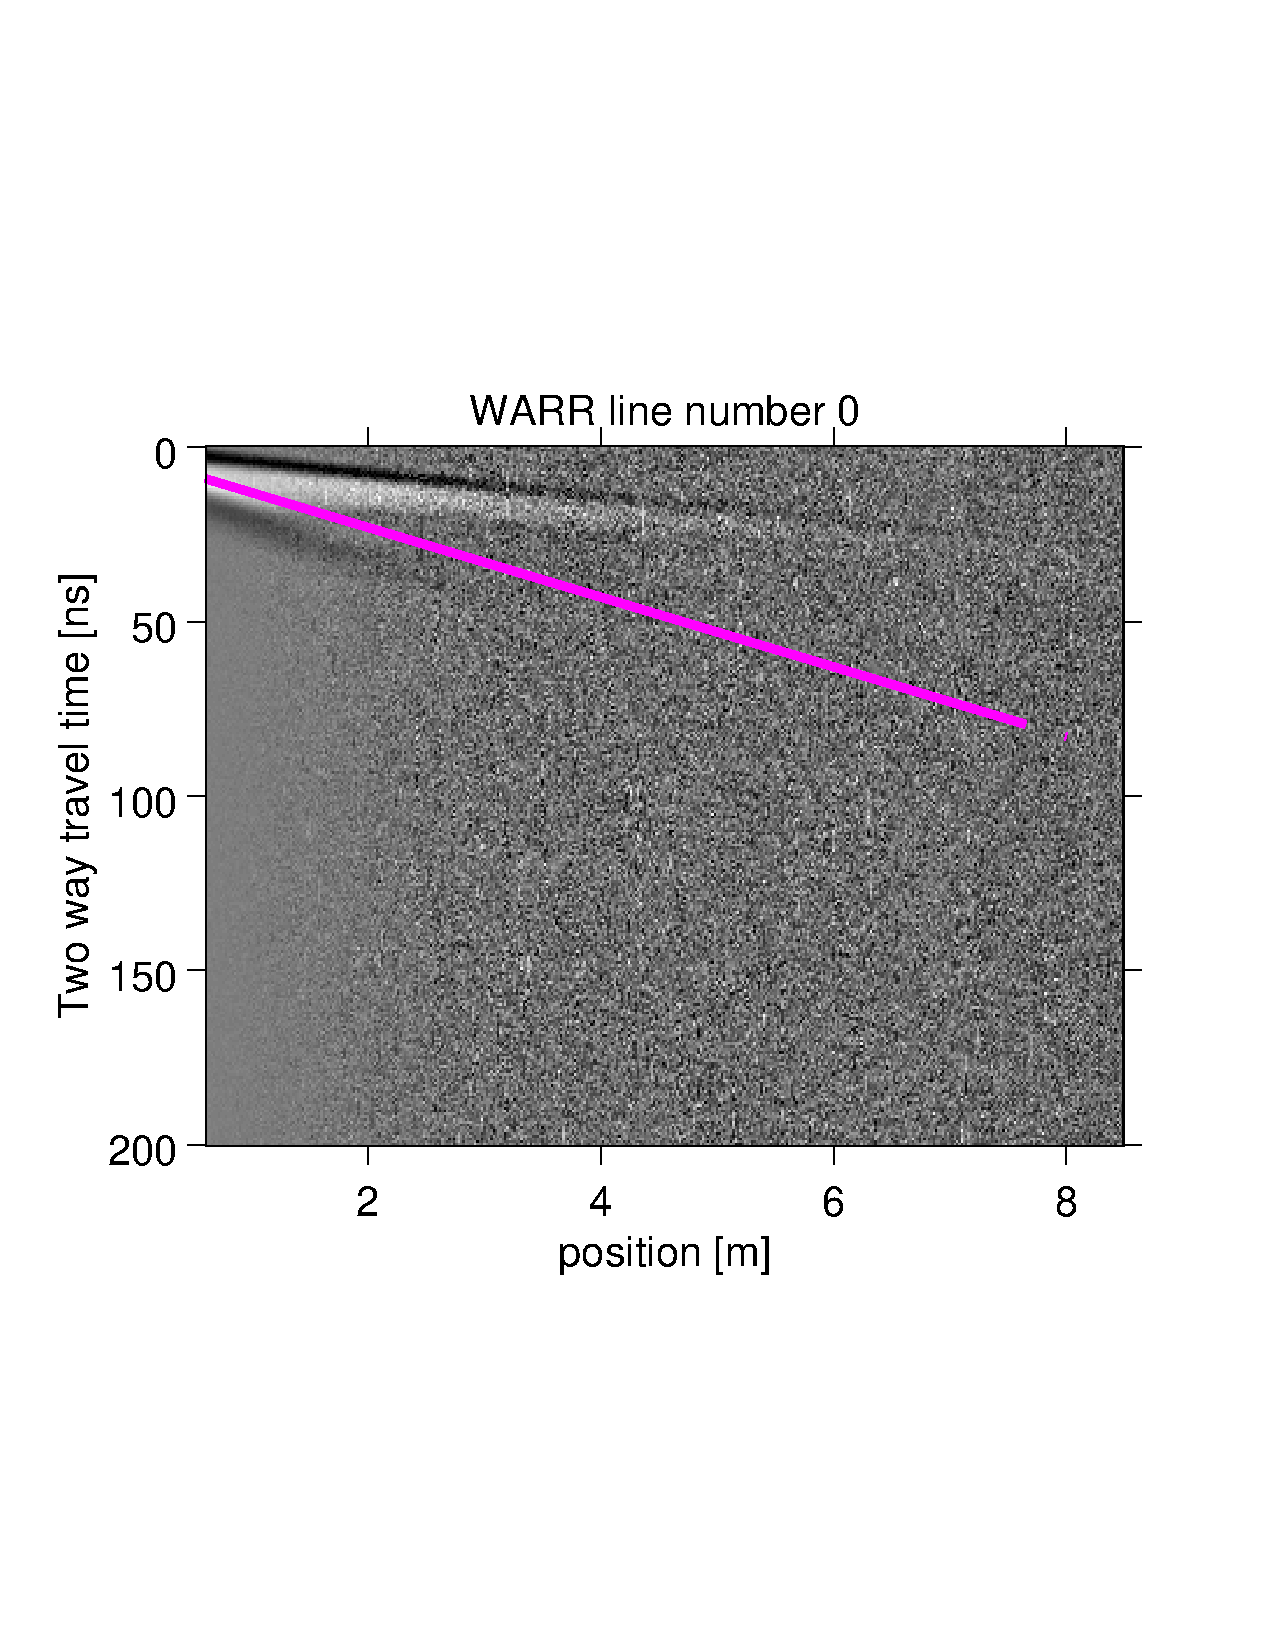
\includegraphics[width=0.7\textwidth, trim = 0.9cm 6cm 2cm
  6.5cm,clip]{figures/WARRrefracted}
\end{center}

It seems as if our guess was not so good. But it is generally very
hard to tell. If only we had a tool that could help us with this. In
fact, we have one. We could just ask our computer to try out many
different such lines and see which ones ``fit'' a line on the WARR
plot. But what does it mean to fit a line on the WARR plot? One
measure of how well a drawn line fits a line on the WARR plot is to
sum up all the pixels along the line. If all pixels have the same
positive or negative value, then their sum will be large. On the other
hand, if our line crosses lines of positive and negative values, or
just runs through noise, then the summands will cancel out and the sum
will be small. Let's do this. The function for it is
\verb#plotWARRrefSemblance#.

Before we continue, let's open a new figure to make sure we do not
half-way overwrite the old one with what's to come. Run

\qquad\verb#figure#

We need to give this program the WARR data, a range for the different
starting two-way travel times, a range for the velocities that it
should test, and the maximum antenna separation we want to consider.

Let's first see how Octave wants us to provide ranges. If we want to
have a list of numbers, between a first number, say 2.3, and a last
number, say 3.1, and we want all the numbers in between with step, say
0.1, then we need to write

\qquad\verb#2.3:0.1:3.1#

So let's say we want to calculate how well all the lines with
starting two way travel times between 0 and 20, step size 0.5, fit
when they have velocities between 0.04 and 0.32 with step size 0.005
and we want to use maximum antenna separation 8 m. Run

\qquad\verb#plotWARRrefSemblance(data,1:0.3:20,0.04:0.003:0.35,8);#

This calculation might take a while. To speed it up you can make the
step size a bit larger but that will also make the resulting image
coarser.

\begin{center}
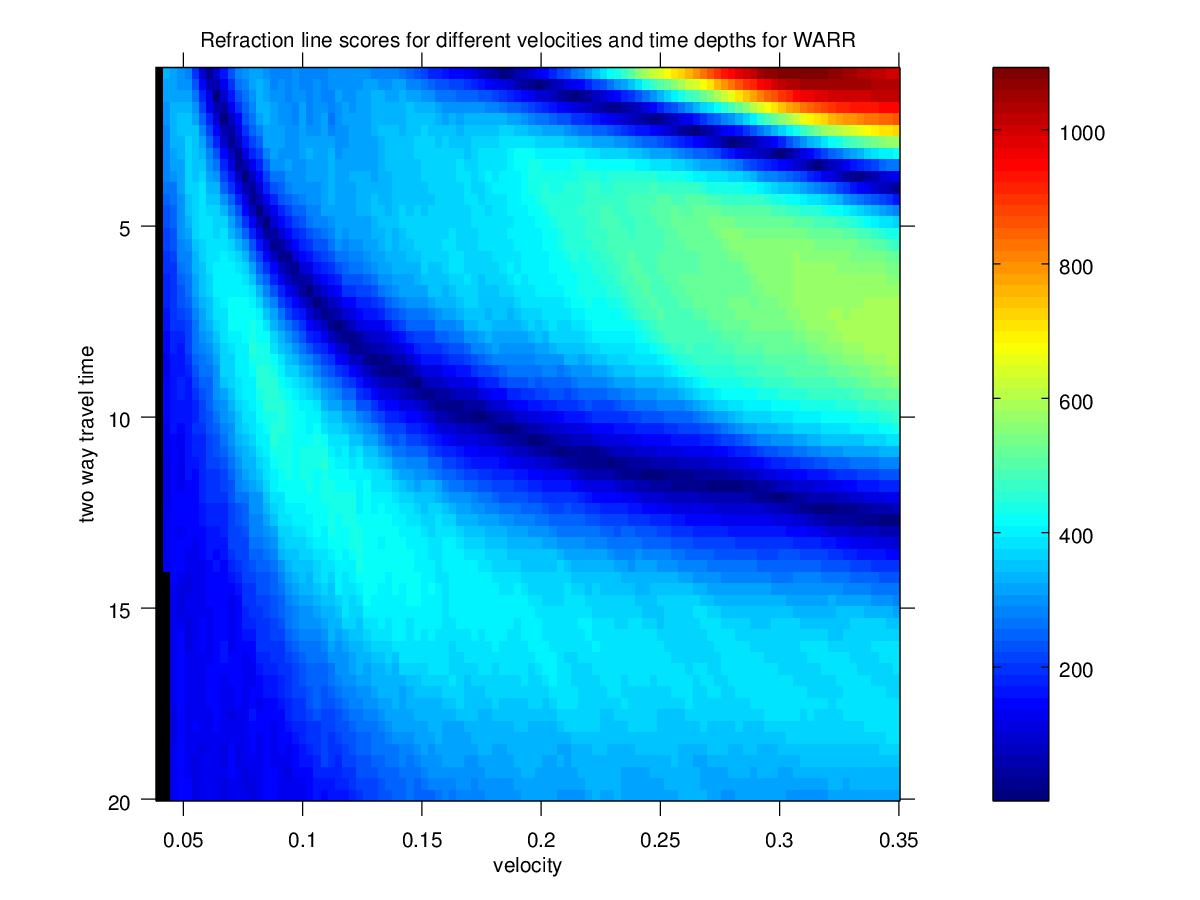
\includegraphics[width=0.7\textwidth, trim = 1cm 0cm 1cm
  0cm,clip]{figures/WARRrefSemblance.jpg}
\end{center}
The x-axis of this plot shows the different velocities that your
computer tested and the y-axis shows the different two-way travel
times at zero antenna distance. Dark-blue means low sum values, so
that means that for these velocity/two-way travel time choices, the
refracted wave lines do not fit any lines in the data. Light blue to
green to red values means that for these choices of velocity/two-way
travel times, the refracted wave lines match a line in the data.

We see three smeared out blobs of good matching. The reason for the
smearing out is that the refracted wave lines in the data are
relatively wide. So even if the chosen refracted wave line is a bit
off, it still lies within the broad actual refracted wave line. Let's
look at the centers of the blobs. When you hover your mouse over the
figure you can read the two-way travel time and velocity values of the
cursor location at the bottom of the figure. The center of the blob at
the top right seems to be for travel time roughly 1 ns and velocity
0.3 m/ns. The second blob seems to be very broad. It's center may be
at around time 6.5 ns and velocity 0.3 m/ns. Finally, the center of
the third blob seems to be at around travel time 9 ns and velocity
0.085.
 
Let's see what these blobs could represent. To do that, let's first
redo the figure with the WARR data:

\qquad \verb#figure#

\qquad \verb#plotWARR(data);#

That's just the WARR data that we already saw. Let's put the
refraction curve corresponding to the first blob on top of this:
 
\qquad \verb#plotWARRrefraction(1,0.3,8);#

It perfectly overlaps with the first black line in the WARR
data. Now the second one:

\qquad \verb#plotWARRrefraction(6.5,0.3,8);#

This one perfectly overlaps with the white line parallel to the black
line. Now the third blob:

\qquad \verb#plotWARRrefraction(9,0.085,8);#

This one follows the black line that was at an angle.

After adding the last line your figure should look like this
\begin{center}
  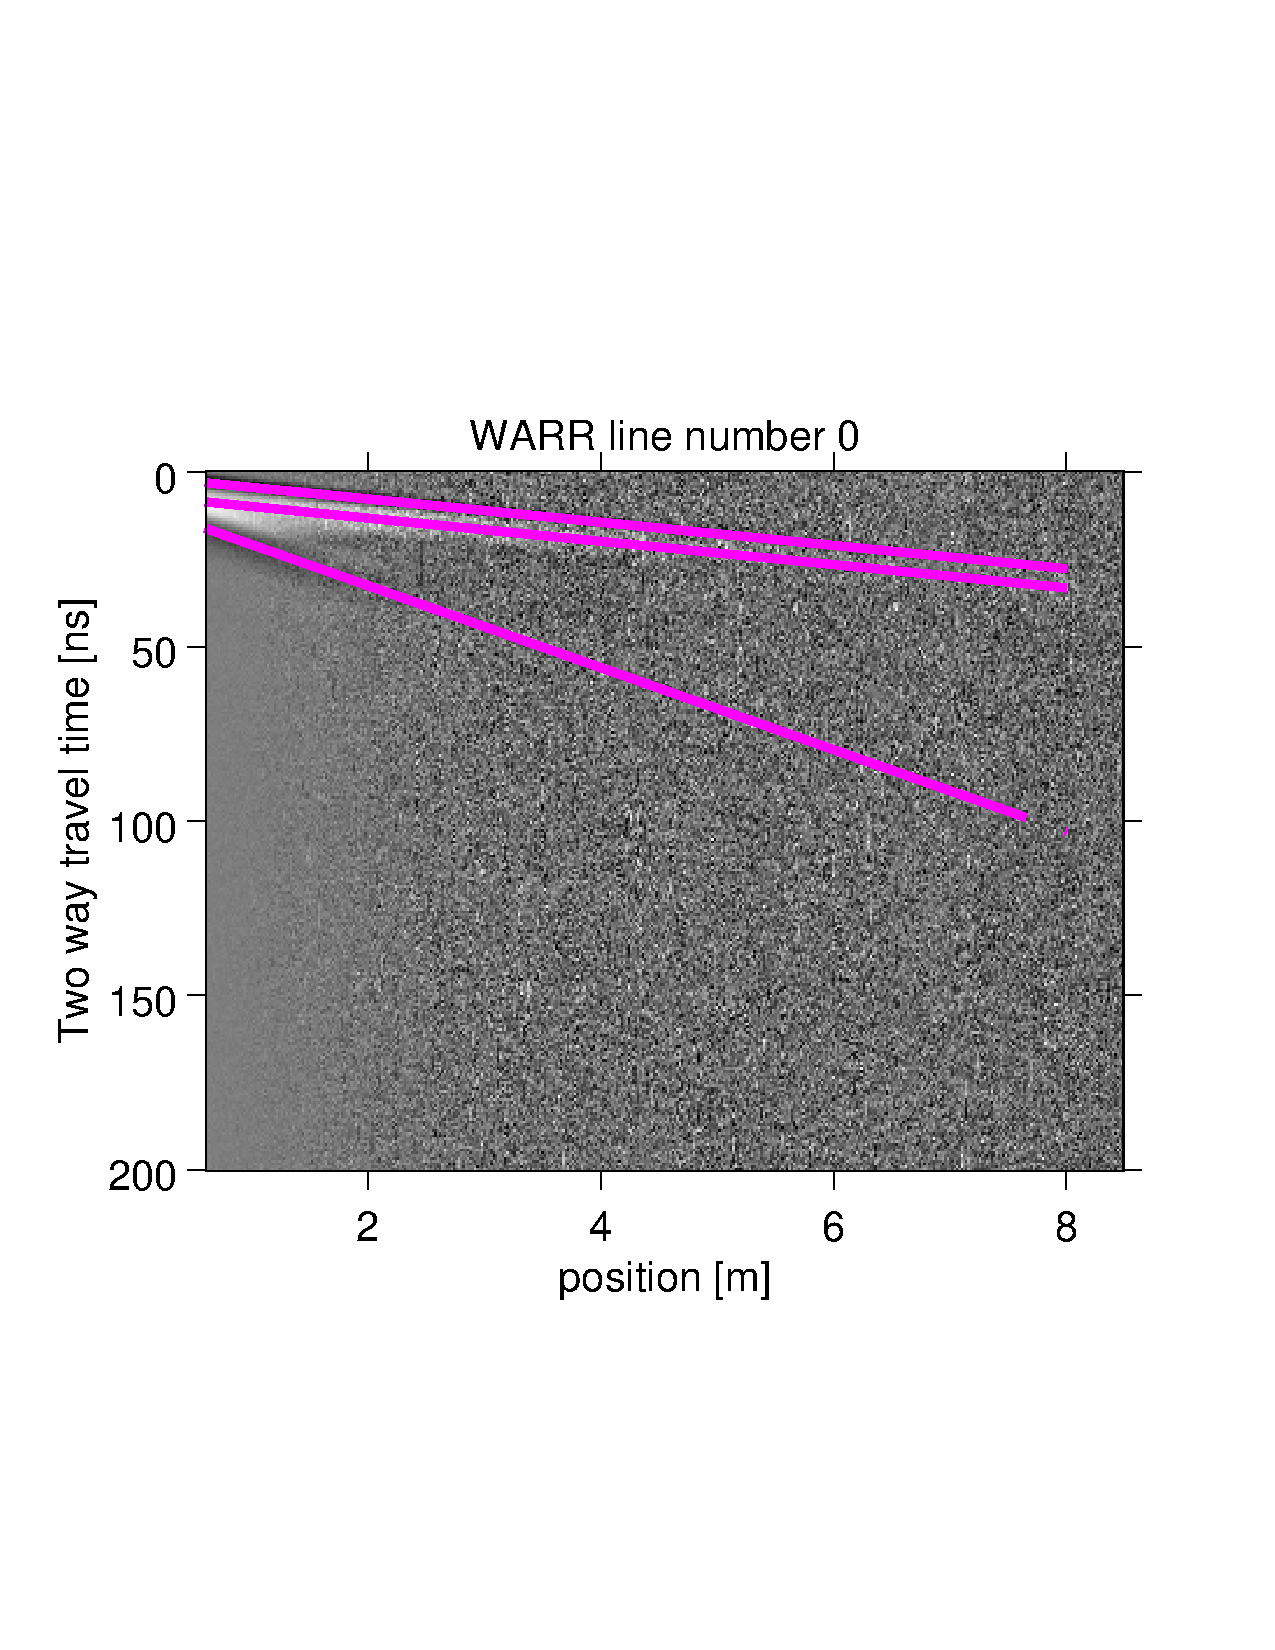
\includegraphics[width=0.7\textwidth,trim = 0.9cm 6cm 2cm
    6.5cm,clip]{figures/WARRlines}
\end{center}

So it looks like we have two refracted waves that travel with velocity
0.3 m/ns and one refracted wave that travels with velocity 0.085
m/ns. The speed of radar waves in air is roughly 0.3 m/s. From this we
know immediately that the first two waves traveled through air and not
through the ground. The separation between them, about 5 ns,
corresponds to the distance 0.3 m/ns * 5 ns = 1.5 m. This is exactly
half the length of the wave in air (3 m). Therefore the ``second''
wave is simply the second lobe of the airwave traveling directly from
the source antenna to the receiver without going through the ground.

The last wave has a velocity of 0.085 m/ns. This is completely within
the normal range we would expect for this type of soil and confirmed
that we were a bit off with our guess from the table. This wave is
called direct wave. It moves just below the surface as a refracted
wave on the air/surface interface.

The question is now: How did we know that these are refracted and not
reflected waves? For reflected waves we would have needed to fit
hyperbolas and use \verb#plotWARRhyperbola# and \linebreak
\verb#plotWARRhypSemblance#.

The answer is: We need to look at the subtle shape of the lines that
we see in the WARR data plot. If these lines bend, then they are
likely to be hyperbolas. If they are straight, then these are either
air- or refracted waves. Another option would be to see what happens
when we use \verb#plotWARRhypSemblance#.  The first two blobs would be
centered at travel time 1.6 ns and velocity 0.28 m/ns, and time 10 ns
and velocity 0.25 m/ns. Both of these velocities are outside of what
we would expect for any type of soil and they would be too slow for
air. The last blob would be centered at velocity 0.07 m/ns and time
14.5 ns, leading to a slightly lower velocity estimation of the
soil. To figure out which of the two velocities: 0.07 or 0.085 we
should trust more, we can look at the hyperbola drawn over the WARR
data and compare it to the refraction line drawn over the WARR data
and see which one we thing fits slightly better:

\qquad \verb#figure#

\qquad \verb#plotWARR(data);#

\qquad \verb#plotWARRhyperbola(14.5,0.07,8);#

\begin{center}
  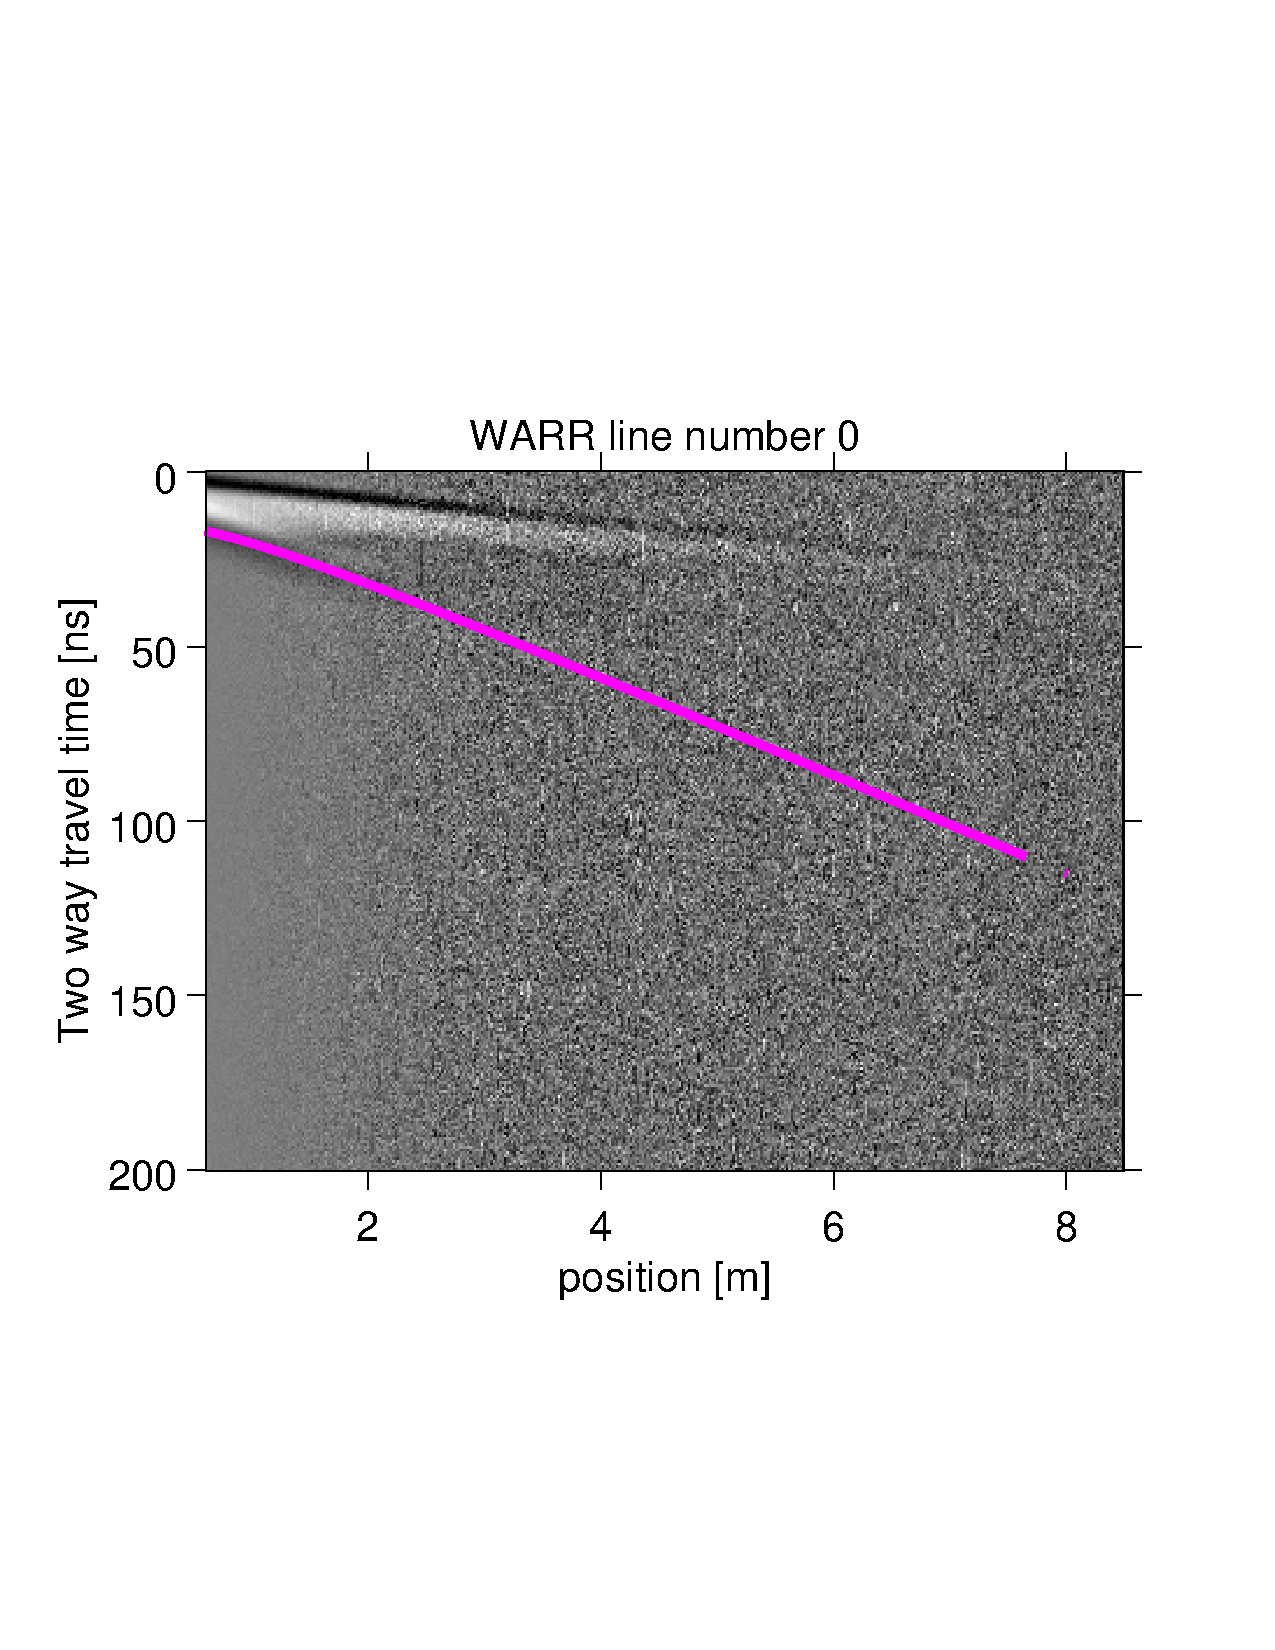
\includegraphics[width=0.7\textwidth,trim = 0.9cm 6cm 2cm
    6.5cm,clip]{figures/WARRhyperb}
\end{center}

It is hard to tell but I think I see that close to the left edge of
the graph, the magenta line curves a bit more than the thick line in
the WARR data.  One approach in such a case of doubt is to give a
depth range of an object based on the two different velocities 0.07
m/ns and 0.085 m/ns.

At this point, in a geophysical investigation, we would go back to the
the GPR profiles in Section~\ref{secProfiles} and replace the velocity
there with the velocities that we just obtained.

\section{Topography}

Realistically, your data will not always be collected on flat terrain. 
GPR-O can account for changes in topography with a two-step process.

First, run

\qquad \verb#makeElev#

\verb#makeElev# prepares an interpolated topography matrix from elevation
values on a grid or along a line (the grid has to have the same spacing on each
line). In other terms, your imported gps data provides elevation points along the profile
that are then connected by interpolation. If your data is 3-D, then ``makeElev''
generates an interpolated surface mesh. 

Next, use the function

\qquad \verb#elevCorrect#

to shift each trace by the (interpolated) corresponding two-way travel
time. 

%I will add a more detailed description at a later point.

\section{Export to VTK}

The function

\qquad \verb#gpro2vtk#

exports GPR-O data to a .vtk file, which can be
read by programs like ParaView etc.

By running

\qquad \verb#help gpro2vtk#

you will see there are six required inputs. For instance, if you
wanted to export the data with AGC gain from the earlier example1, run

\qquad \verb#gpro2vtk(dataHGa,0.06,0.2,0,'Exercise1Data',[]);#

Programs like Paraview offer powerful 3-D visualization of data.
Here is a quick example of the exported data, represented in Paraview.

\begin{center}
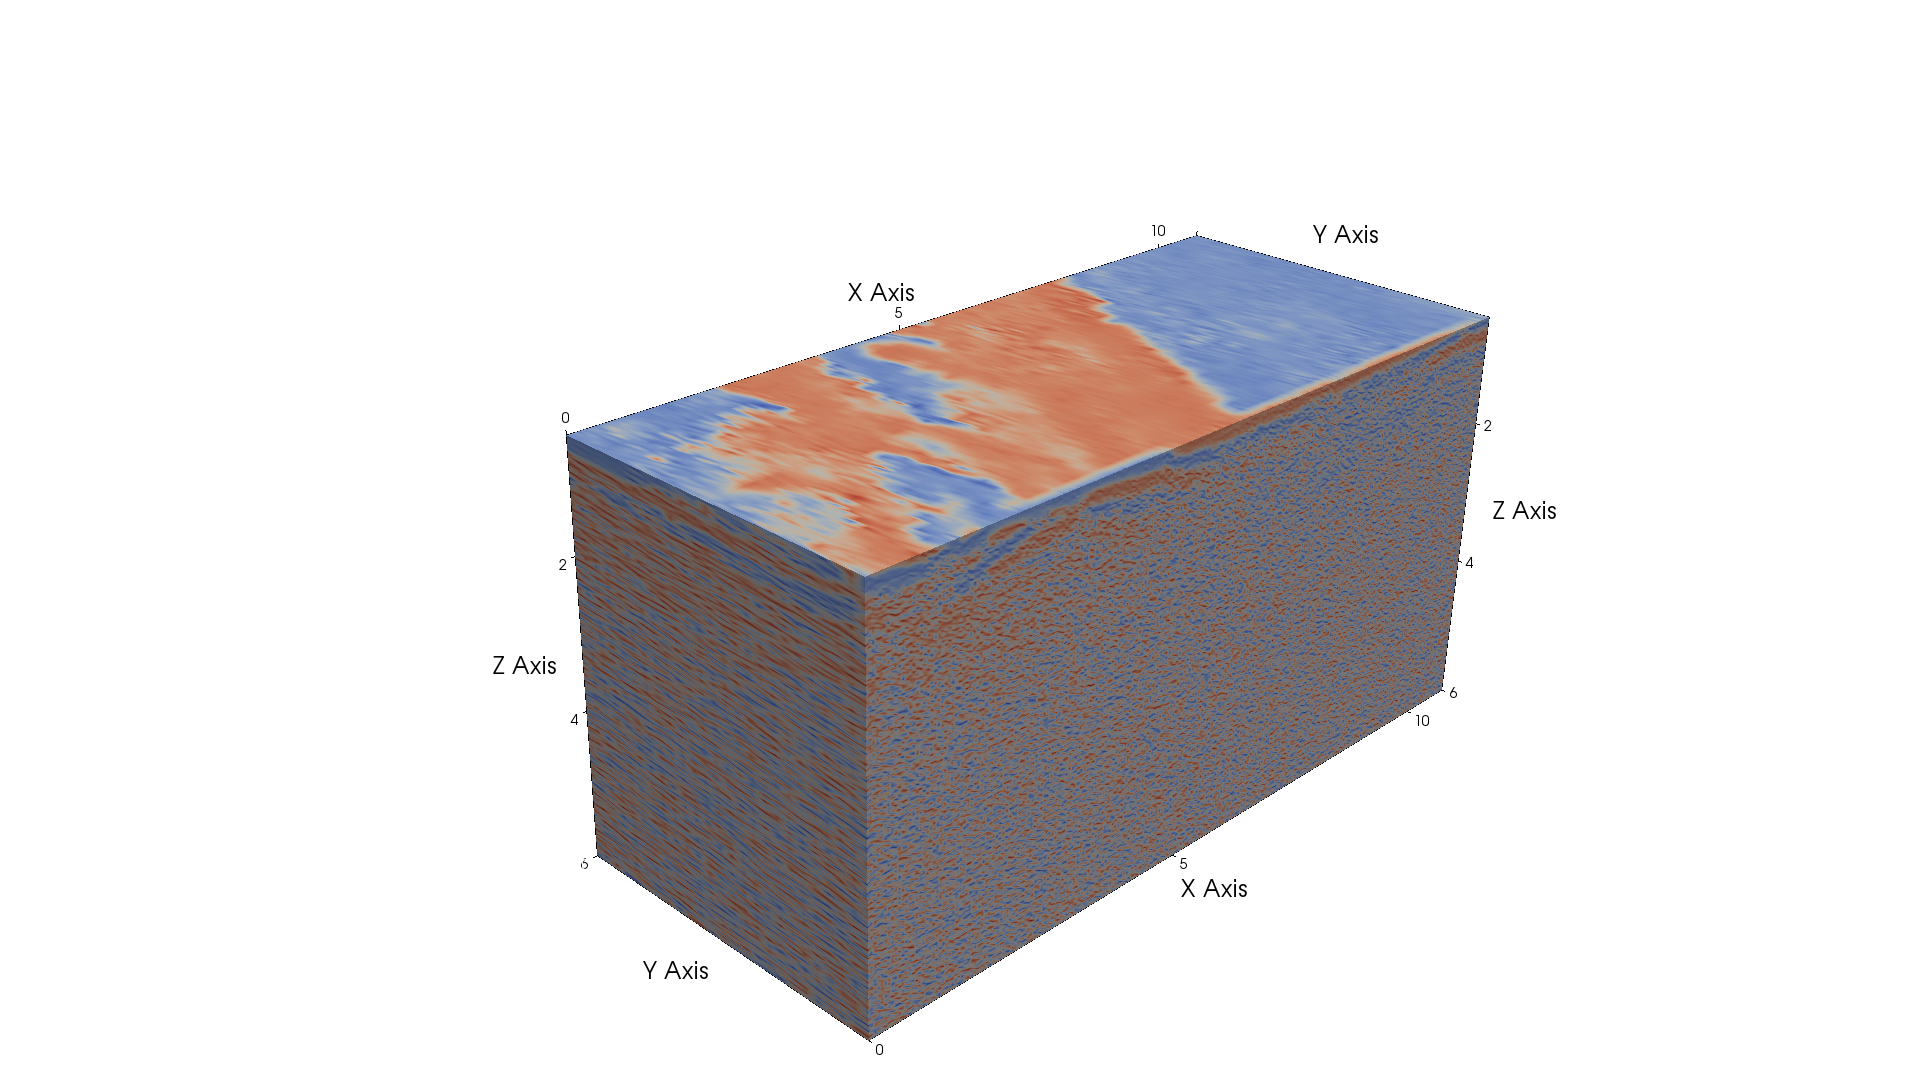
\includegraphics[width=0.7\textwidth, trim = 1cm 3cm 1cm
  3cm,clip]{figures/ParaviewEx.png}
\end{center}

\section{Other potentially useful functions}

The function

\qquad \verb#thresh#

removes values smaller than a percentage of the maximum data point
value. In the default GPR profiles we compiled in this documentation,
note how the signals (and noise) lie on the greyscale color spectrum. The
stronger (black or white) bands are generally the strongest signals,
while the noise is usually averaged out as grey. This function reduces
the grey by setting small deviations to zero. This can be used to 
clean up traces before gain and export to VTK.

The function

\qquad \verb#stolt_fk_mig#

is a migration tool that removes artifacts within GPR profiles that are
caused by changing the receiver-transmitter position. The reason that a
reflection point in the subsurface generates a parabolic arc in radargrams
is that the two-way distance to a point increases when the antennas are moved
further from the point in both directions. By incorporating this relationship
within our processing, we can improve the accuracy of the GPR profile.

The function

\qquad \verb#readSnS_GPS# 

reads Sensors and Software GPS data, such as the one provided by 
\url{https://alaska.usgs.gov/portal/project.php?project_id=384} 

\end{document}
